\documentclass[12pt]{article}

\setlength\parindent{30pt}
\usepackage[usenames, dvipsnames]{color}
\usepackage{fullpage}
\usepackage{setspace}
\usepackage{amssymb}
\usepackage{amsmath}
\usepackage{caption}
\usepackage{subcaption}
\usepackage{graphicx}

\usepackage[utf8]{inputenc}
\usepackage[T1]{fontenc}

% \doublespacing

\usepackage[style=authortitle-ticomp, natbib=true, backend=biber]{biblatex}
% \usepackage[style=authoryear-ibid, natbib=true, backend=biber]{biblatex}
\addbibresource{sources.bib}

\newcommand{\TODO}[1]{\textcolor{red}{#1}}
\newcommand{\F}[1]{\textcolor{magenta}{#1}}

\newcommand{\contradiction}{{\hbox{%
      \setbox0=\hbox{$\mkern-3mu\times\mkern-3mu$}%
      \setbox1=\hbox to0pt{\hss$\times$\hss}%
      \copy0\raisebox{0.5\wd0}{\copy1}\raisebox{-0.5\wd0}{\box1}\box0
    }}}


\newcommand\Nbb{\mathbb{N}}
\newcommand\Pbb{\mathbb{P}}
\newcommand\Zbb{\mathbb{Z}}
\newcommand\Rbb{\mathbb{R}}
\newcommand\Mcl{\mathcal{M}}

\begin{document}
\title{CMSC 324}
\author{Patrick Collins, Zachary Jenkins \& Mark Landgrebe}
\date{\today}
\maketitle
\pagebreak

\section{Contact Info}
Team Name: PlayListr

\begin{center}
\begin{tabular}{l|l}
 Member           &  Email                    \\ \hline
 Patrick Collins  &  pscollins@uchicago.edu   \\
 Zachary Jenkins  &  zjenkins@uchicago.edu    \\
 Mark Landgrebe   &  mlandgrebe@uchicago.edu  \\
\end{tabular}
\end{center}

\pagebreak

\section{Motivation}

\pagebreak
\section{Background}

\pagebreak

\section{Project Specification}
The fundamental purpose of PlayListr is to improve the experience of
guests at events playing music. However, there are a variety of
avenues by which we can achieve this goal, and we hope to explore as
many of them as we can under the time constraints.

\subsection{Capabilities}
We can divide our planned features in to a hierarchy, such that each
higher level depends upon a correct implementation of the previous
one:

\begin{enumerate}
\item Core functionality.

The core functionality of the app is to allow a host to create a ``room,''
and to allow guests who join the room to have control over the music
that is played.

However, a variety of structure must be in place in order to
accomplish this goal. The core functionality is the most ambitious
part of this project --- a successful implementation requires:
\begin{itemize}
\item Correct interoperation with Spotify in order to authenticate
  users and stream music.
\item Construction of a database to hold identifying information about
  users, with sufficient information to reconstruct the user's Spotify
  account details, as well as the details of all existing rooms and
  the songs enqueued within them.
\item Development of a server that exposes a REST API, giving access
  to the database and allowing simple CRUD operations.
\item Ensuring consistency across many mobile users connected to the
  same room, taking in to account the possibility of high network
  latency over cellular data networks.
\end{itemize}

With this in mind, we have focused our current development efforts on
building the core functionality before tackling the features that
follow --- in the ``software architecture'' section below, we outline
an implementation of the core functionality.

\item Location awareness.

Users should be prompted to join a room whenever they come within a
pre-set distance of an existing room via push notification.

\item Smartwatch integration.

  Users should be able to vote on songs and see the currently playing
  song from the display of their Android smartwatches. This will
  likely take place via Bluetooth communication with their
  smartphones. This step is crucial for the following step since
  smartwatch sensor data will allow for a much more accurate picture
  of user activity within a room.

\item Adaptive song selection on the basis of sensor data.

The app should detect when the activity level within a room rises or
falls and play faster- or slower-paced music, accordingly. For
simplicity, we will simply select songs currently in the queue and pad
tempo-matched songs with artificial votes in order to float them to
the top of the queue --- this avoids problems of trying to match the
genre of the music currently being played.

We can take a variety of angles in processing sensor data, but the
simplest is likely to be taking the average norm of the acceleration
vector of each user per unit time. For example, given that we have
accelerometer data for the user's acceleration $\vec{a}$ such that:
\[
\vec{a} = (x, y, z)
\]
And, letting $\vec{a}_u$ represent the acceleration vector for the user
$u$ belonging to the group of users $U$ in a room during the previous
tick, we define the activity level $l$ of that tick to be:
\begin{align*}
  l &= \sum_{u \in U} \frac{||\vec{a}||}{|U|}\\
  &= \sum_{u \in U} \frac{\sqrt{x^2 + y^2 + z^2}}{|U|}
\end{align*}
Yielding a natural and intuitive notion of ``activity level'' that can
be quickly computed.


\item Social features.

Users have a ``friend list,'' consisting of other users, that allows
them to initiate communication (perhaps via a builtin messaging
service, or a tie in to an external messaging service, such as
Facebook Messenger).

\item Gesture recognition.

Users can add each other to their friend lists by shaking hands. Time
permitting, we can explore other gestures, such as a high five to
indicate that both users upvote the current song.

\item User pairing on the basis of activity level.

Given that the server will have access to the activity levels of all
users in a room, users can opt-in to a ``friendly mode'' in which they
will be periodically asked if they would like to become friends with
another user in the room based on similar activity levels (and perhaps
similar music preferences). If both users accept, then a conversation
is initiated between the two.

\end{enumerate}

\subsection{Software Architecture \& Design}
\begin{figure}[h]
  \centering
  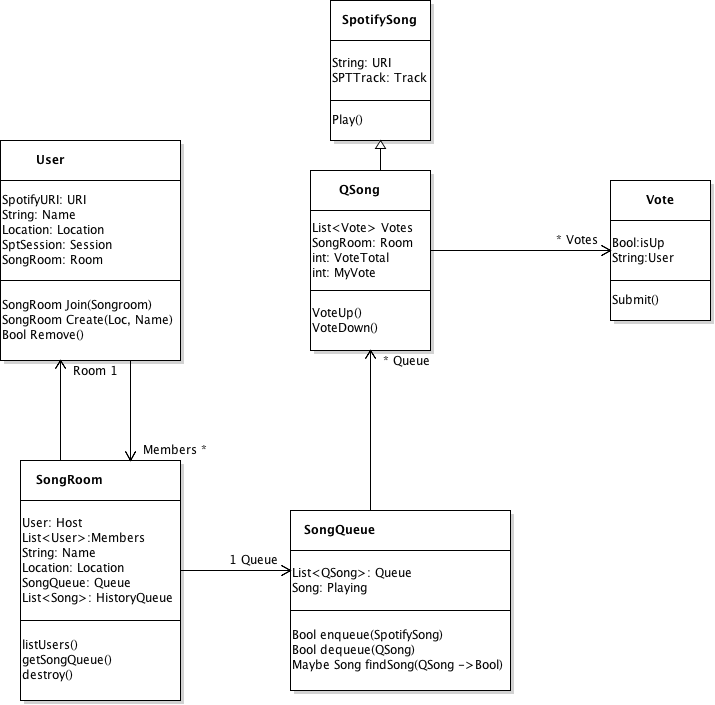
\includegraphics[width=4in]{ClassDiagram}
  \caption {UML Diagram of Client-Side Code}
\end{figure}

\begin{figure}[htb!]
  \centering
  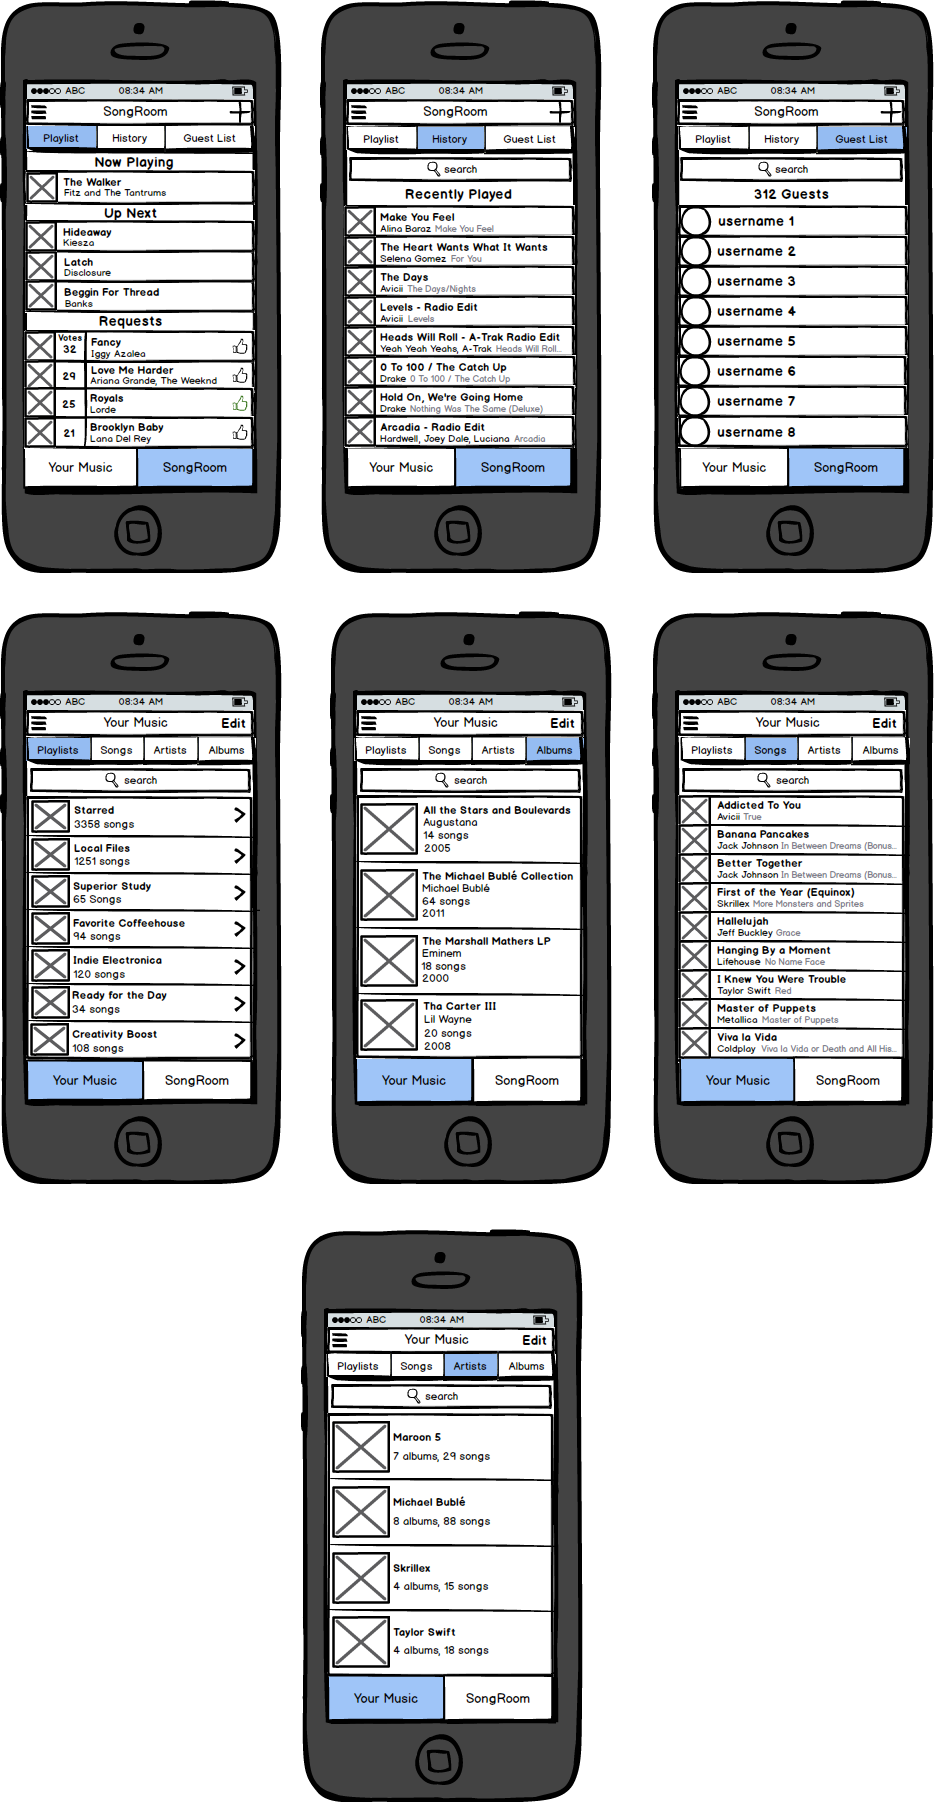
\includegraphics[width=4in]{mockup.png}
  \caption {UI Mockup}
\end{figure}

\begin{figure}[htb!]
  \centering
  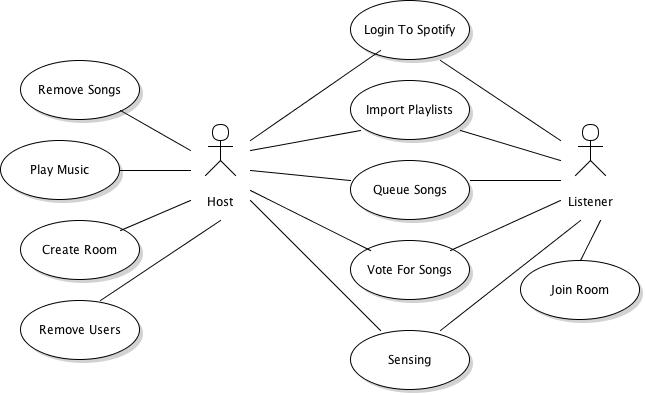
\includegraphics[width=4in]{usecase-diagram}
  \caption {Use Case Diagram}
\end{figure}


\pagebreak

\section{Planned Demonstration}

\pagebreak

\section{Implementation Schedule \& Supporting Tools}



\end{document}
